% Created 2024-08-03 Sat 16:23
% Intended LaTeX compiler: pdflatex
\documentclass[10pt]{article}
% =================================BASE====================================%
\usepackage[left=2cm,right=2cm,top=2cm,bottom=2cm]{geometry} % Marges
\usepackage[T1]{fontenc} % Nécessaire avec FrenchBabel
\usepackage[utf8]{inputenc} % Important pour symboles Francophones, é,à,etc
\usepackage{csquotes} % Recommandé par PDFLatex lors de la compilation. 

% Calligraphie
%\usepackage{pxfonts} % Met le texte ET les maths en Palatino + donne accès à des symboles math
%\usepackage{palatino} % Cette commande met seulement le texte en police palatino
\usepackage{lmodern} % Pour les maths? Lmodern pour les maths
\usepackage{cfr-lm}
% Use lmodern for sans-serif
\usepackage{mathrsfs} % Permet la command \mathscr (Lettres attachées genre) \mathscr(B)

% Bibliographie
%\usepackage[backend=bibtex,style=phys,sorting=ynt]{biblatex}
\usepackage[backend=biber,sorting=ynt,style=authoryear]{biblatex} % N'est pas utilisé par le compilateur org-mode, mais NÉCESSAIRE. Voir le fichier init.el pour changer le style. 



\usepackage{amsmath, amssymb, amsthm} % Symb. math. (Mathmode+Textmode) + Beaux théorèmes.
\usepackage{mathtools,cancel,xfrac} % Utilisation de boîtes \boxed{} + \cancelto{}{}, xfrac
\usepackage{graphicx, wrapfig} % Géstion des figures.
\usepackage{hyperref} % Permettre l'utilisation d'hyperliens.
\usepackage{color} % Permettre l'utilisation des couleurs.
\usepackage{colortbl} % Color tables
\usepackage[dvipsnames]{xcolor} % Couleurs avancées.

% Physique
\usepackage{physics} % Meilleur package pour physicien. 

% Style
\usepackage{lipsum} % For fun
\usepackage{tikz} % Realisation de figures TIKZ.
\usetikzlibrary{arrows.meta,bending} % Arrow heads 
\usepackage{empheq} % Boite autour de MULTIPLE équations
\usepackage{bbding}

% Français
\usepackage[french]{babel} % Environnements en Français.

\usepackage{titling} % Donne accès à \theauthor, \thetitle, \thedate

% ==============================BASE-(END)=================================%





% ================================SETTINGS=================================%
% Pas d'indentation en début de paragraphe :
\setlength\parindent{0pt}
\setlength{\parskip}{0.15cm}

% Tableaux/tabular
% Espace vertical dans les tabular/tableaux
\renewcommand{\arraystretch}{1.2}
% Couleur des tableaux/tabular
% \rowcolors{3}{violet!5}{}

% Couleurs de hyperliens :
\definecolor{mypink}{RGB}{147, 0, 255}
\hypersetup{colorlinks, 
             filecolor=mypink,
             urlcolor=mypink, 
             citecolor=mypink, 
             linkcolor=mypink, 
             anchorcolor=mypink}


% Numéros d'équations suivent les sections :
\numberwithin{equation}{section} 

% Les « captions » sont en italique et largeur limitée
\usepackage[textfont = it]{caption} 
\captionsetup[wrapfigure]{margin=0.5cm}

% Retirer l'écriture en gras dans la table des matières
\usepackage{tocloft}
\renewcommand{\cftsecfont}{\normalfont}
\renewcommand{\cftsecpagefont}{\normalfont}

% Change bullet style
\usepackage{pifont}
\usepackage{enumitem}
%\setlist[itemize,1]{label=\ding{224}}
\setlist[itemize,1]{label=\ding{239}}
\renewcommand{\boxtimes}{\blacksquare}
% ================================SETTINGS=================================%



% ==============================NEWCOMMANDS================================%
% CQFD symbol
\renewcommand{\qedsymbol}{$\hfill\blacksquare$}

% Vecteurs de base :
\newcommand{\nvf}{\vb{\hat{n}}}
\newcommand{\evf}{\vb{\hat{e}}}
\newcommand{\ivf}{\vb{\hat{i}}}
\newcommand{\jvf}{\vb{\hat{j}}}
\newcommand{\kvf}{\vb{\hat{k}}}
\newcommand{\uu}{\vb{u}}
\newcommand{\vv}{\vb{v}}
\newcommand{\ust}{\vb{u}_{\ast}}

% Physics empty spaces 
\newcommand{\short}{\vphantom{pA}}
\newcommand{\tall}{\vphantom{pA^{x^x}_p}}
\newcommand{\grande}{\vphantom{\frac{1}{xx}}}
\newcommand{\venti}{\vphantom{\sum_x^x}}
\newcommand{\pt}{\hspace{1pt}} % One horizontal pt space

% Moyenne numérique entre deux points de grilles. 
\newcommand{\xmean}[1]{\overline{#1}^x}
\newcommand{\ymean}[1]{\overline{#1}^y}
\newcommand{\zmean}[1]{\overline{#1}^z}
\newcommand{\xymean}[1]{\overline{#1}^{xy}}

% Tilde over psi
\newcommand{\tpsi}{\tilde{\psi}}
\newcommand{\tphi}{\tilde{\phi}}

% Nota Bene env : (\ding{89})
%\newcommand{\nb}{$\boxed{\text{\footnotesize\EightStarConvex}\pt \mathfrak{N. B.}}$\hspace{4pt}}
\newcommand{\nb}{\underline{{\footnotesize\EightStarConvex}\pt $\mathfrak{N.B.}$\vphantom{p}}\hspace{3pt}}

\newcommand{\exemple}{
\parbox[center]{2.2cm}{\begin{tcolorbox}[sharp corners, rounded corners=northeast, rounded corners=southeast,
colback=Violet!2, colframe=black,
size=small, width=2cm, left=-0.25pt, bottom=-0.5pt,
arc is angular, arc=2.5mm, boxrule=0.35pt, leftrule=4pt, %bottomrule=1pt,
after={\enskip}] Exemple \end{tcolorbox}}}

\newcommand{\rad}{\text{Rad}}


\newcommand{\cqfd}{\hfill$\blacktriangleleft$}

% Define the nota bene environment
\usepackage{tcolorbox}
\newtcolorbox{notabene}{
     colback=blue!5,
     colframe=black,
     boxrule=0.5pt,
     arc=2pt,
     left=5pt,
     right=5pt,
     top=5pt,
     bottom=5pt,
}


\newcommand{\cmark}{\ding{52}}
\newcommand{\xmark}{\ding{55}}
% ==============================NEWCOMMANDS================================%



% ==============================PAGE-TITRE=================================%
% Titlepage 
\newcommand{\mytitlepage}{
\begin{titlepage}
\begin{center}
{\Huge \thesubtitle \par}
\vspace{2cm}
{\Huge \MakeUppercase{\thetitle} \par}
\vspace{2cm}
RÉALISÉ DANS LE CADRE\\ D'UN PROJET POUR \par
\vspace{2cm}
{\Huge ISMER--UQAR \par}
\vspace{2cm}
{\thedate}
\end{center}
\vfill
Rédaction \\
{\theauthor}\\
\url{charles-edouard.lizotte@uqar.ca}\\
ISMER-UQAR\\
Police d'écriture : \textbf{CMU Serif Roman}
\end{titlepage}
}
% ==============================PAGE-TITRE=================================%



% =================================ENTÊTE==================================%
\usepackage{fancyhdr}
\pagestyle{fancy}
\setlength{\headheight}{13pt}
\renewcommand{\headrulewidth}{0.025pt} % Ligne horizontale en haut

\fancyhead[R]{\textit{\thetitle}}
\fancyhead[L]{\ \thepage}
\fancyfoot[R]{\textit{\theauthor}}
\fancyfoot[L]{}
\fancyfoot[C]{} 
% =================================ENTÊTE==================================%
\author{Charles-Édouard Lizotte}
\date{17/03/2023}
\title{Rapport hebdomadaire -- McGill}
\newcommand{\thesubtitle}{Contrat Été 2023}
\hypersetup{
 pdfauthor={Charles-Édouard Lizotte},
 pdftitle={Rapport hebdomadaire -- McGill},
 pdfkeywords={},
 pdfsubject={},
 pdfcreator={Emacs 29.4 (Org mode 9.7.8)}, 
 pdflang={French}}
\begin{document}

\mytitlepage
\tableofcontents\newpage
\section{Le modèle est en état de fonctionner [2/2]}
\label{sec:org7d6a018}
\subsection{Mise en contexte}
\label{sec:org89c8df5}
Avant de débuter les changements au modèle \emph{shallow water}, assurons nous 
\begin{enumerate}
\item qu'il est compilable;
\item qu'il peut rouler sans erreur sur toutes les machines (donc qu'on n'utilise pas des routine Fortran trop vieilles, entre autre).
\end{enumerate}
Au cours de ma maîtrise, quelques petits problèmes conceptuels et techniques s'étaient déjà accumulés au fil du code.
Nous allons donc régler ces problèmes-là et s'assurer que tout marche, avant tout. 
\subsection{{\bfseries\sffamily DONE} Régler le problème des \emph{oldfile}}
\label{sec:orgb974324}
Comme on avait couplé le modèle \emph{shallow water} avec Wavewatch III dans le passé, les \emph{restart files} devaient avoir une forme légèrement différente que dans la version de Tianze.
Principalement, il fallait ajouter la dérive de Stokes du dernier pas de temps \textbf{à l'intérieur du restart file}.
À l'époque, la solution que j'avais trouvé était de rajouter une \emph{switch} nommée \textbf{oldfile} dans le fichier de paramètres, \emph{parameter.f90}.
Ceci avait comme problématique la coexistence de deux types de \emph{restart files} un peu partout. 
Ça augmentait malheureusement le risque d'erreurs à chaque fois qu'on relançait des expériences, mais ça m'évitait de devoir relancer mes plus longues expériences -- qui contenaient souvent des résultats importants.
C'était une solution temporaire qui s'est malheureusement éternisée jusqu'à la fin de la maîtrise. 
\textbf{Je me met une note} qu'on devrait toujours avoir les mêmes type de \emph{restart files} pour éviter d'avoir \textbf{beaucoup trop} de \emph{switches}.\\

Comme solution, couplé ou non, les \emph{restart files} vont maintenant contenir la dérive de Stokes et le dernier \(\tau\) à la surface de l'eau.
Et puis, la \emph{switch} \textbf{oldfile} a tout simplement été retirée, maintenant qu'on a supprimé ces vieilles données-là.
\subsection{{\bfseries\sffamily DONE} Régler le bordel des \emph{compile model} et recompiler efficacement}
\label{sec:orgf6e103b}
Un lecteur avisé de mon mémoire aurait remarqué la présence de 3 modèles différents.
Le tout avec de nombreux fichiers de paramètres associés à chacun.
C'est pourquoi, lors de ma maîtrise, j'ai du codé plusieurs compilateurs avec plusieurs dossiers et plusieurs listes différentes de paramètres.
Avec le temps, le nombre de compilateurs a grandit de manière exponentielle dans mes dossiers, il a donc fallu faire un gros ménage juste pour faire  fonctionner le modèle \emph{shallow water} sur mon portable.
Comme  les différentes librairies Fortran ne sont pas les même sur mon ordinateur, il a fallut reconstruire un compilateur.
Mais ça fonctionne maintenant à la perfection!\\


Par précision, il a fallu installer les librairies à l'aide des commandes
\begin{verbatim}
sudo apt-get install libfftw3-dev libfftw3-doc
\end{verbatim}
et pour trouver le \emph{path},
\begin{verbatim}
dpkg -L libfftw3-bin
\end{verbatim}
ce qui nous permet d'ajouter
\begin{verbatim}
fftw_path=/usr/share/doc/libfftw3-bin/
\end{verbatim}
à motre \emph{makefile} (\emph{compile model} dans notre cas). 
Pour l'instant, la compilation fonctionne; j'ai lancé un test pour la nuit ce \textit{<2023-03-14 Tue>}.\\

\textbf{Pour que le modèle roule bien}, mentionnons qu'il a besoin de certains dossiers et fichiers, soit 
\begin{itemize}
\item tous les fichiers texte associés aux nombres d'onde;
\item les dossiers \emph{data} et \emph{specdata} vides pour les donneés;
\item un dossier \emph{rst} vide pour les \emph{restart files}.
\end{itemize}
J'ai donc créé un fichier vide prêt à partir.
\section{Modifications à apporter au modèle \emph{shallow water} cette semaine [1/1]}
\label{sec:org104ccb4}
\subsection{{\bfseries\sffamily DONE} Retirer la \emph{slab layer}}
\label{sec:org87283a5}
Comme on veut un modèle à plusieurs couches, la \emph{slab layer} ne sert plus vraiment à rien.
Aussi, comme on veut nettoyer le code, retirer la \emph{slab layer} est probablement la première chose à faire. 
Déjà, Ça va nous débarrasser de quelques sous-routines superflues et beaucoup de variables maintenant inutiles.\\

J'ai ajouté la quantité \textbf{UStokes} et \textbf{VStokes} dans les sous-routines \emph{p corrections.f90} et \emph{rhs.f90} (avec un top(k)), de sorte que ça apparaisse dans le \emph{RHS} de la conservation de la masse et pour le gradient de pression à la surface. 
Bref, cette quantité couplée a simplement remplacé \emph{Uek} et \emph{Vek} dans les deux même sous-routines.
\textbf{UStokes} et \textbf{VStokes} sont définis comme nulles dans la sous-routine \emph{initialize.f90} et ne sont pas mises à jour sans l'activation de \emph{switch} (COU .eq. .true.), qui permet le couplage avec le modèle de vagues.\\

J'ai aussi profité de cette occasion pour alléger les lignes de codes liées au \(\tau_o\) à la surface. 
Avant, j'avais deux \emph{switches} pour choisir si le transfert de momentum de l'atmosphère devait être sur la première couche, la couche d'Ekman ou couplée avec Wavewatch III.
Bref, c'était un bordel et j'en ai profité pour faire un un gros ménage dans tous ces \emph{switches} là.
Ça pourrait expliquer pourquoi tout ça me prend un peu plus de temps que prévu, disons\ldots{}\\

Finalement, toutes les sous-routines \emph{dump etc.f90} -- que Tianze avait rajoutées -- ont pris beaucoup de temps à réorganiser.
Dans chacune d'elles, il y avait un \emph{Uek} qui était couplé avec d'autres quantités qui servaient de diagnostique, etc.
Dans le même ordre d'idée, le courant est maintenant exporté avec la même \textbf{shape} que tous les autres champs.
Avant, le courant de \textbf{toutes les couches} était exporté dans le même fichier avec le préfixe \emph{u\textsubscript{o}} (pour le différentier de \emph{Uek}). 
Maintenant, ce sera \emph{u\textsubscript{1}}, \emph{u\textsubscript{2}}, \emph{u\textsubscript{3}}, etc.
De cette manière, ma fonction Python (\textbf{readata.py}) qui ouvre les \emph{output} du modèle \emph{shallow water} pour les transformer en fichier \textbf{NetCDF} va seulement ouvrir des fichiers de même taille.
C'est quelque chose que je n'avais pas entrepris pendant ma maîtrise, car je n'ai simplement pas eu le temps pendant ma rédaction.
Je suis bien heureux que ça soit enfin fait.
Essentiellement, le modèle commence à être bien plus \emph{clean}, pour reprendre les mots de David.\\

Toujours vers la fin de la semaine, le modèle semble encore \emph{exploser}, comme la fameuse ligne \emph{thickness too small} aime si bien nous le rappeler. 
Ce vendredi, j'ai investigué et il semble que ce soit parce que le transfert de momentum depuis l'atmosphère est définit comme 
\begin{equation}
\tau_0 = \frac{\tau_{atm}}{\rho_o},
\end{equation}
ce qui voulait dire que j'envoyais des vents de l'ordre de 1000 m/s au modèle.
Pour information, on lance la même expérience que (Chen et al, 2021), mais avec seulement deux couches, ce qui pourrait s'apparenter à si \(H_{Ek} = H_1\).

\begin{table}[htbp]
\caption{Valeur des différents paramètres de l'expérience de Chen et al (2021).}
\centering
\begin{tabular}{lll}
\hline
\hline
Paramètres & Symbole & Valeur\\
\hline
Taille du domaine & L\textsubscript{x} = L\textsubscript{y} & 2000 km\\
Pas de temps & \(\Delta\) t & 300 s\\
Paramètre de Coriolis & f & 7\texttimes{}10\textsuperscript{-5} s\textsuperscript{-1}\\
Amplitude du vent & \(\tau\)\textsubscript{atm} & 0.1 N m\textsuperscript{-2}\\
Coefficient de viscosité biharmonique & A\textsubscript{bh} & dx\textsuperscript{4} \texttimes{}10\textsuperscript{-5} s\textsuperscript{-1}\\
Coefficient de frottement au fond & r\textsubscript{drag} & 10\textsuperscript{-7} s\textsuperscript{-1}\\
Coefficient dissipation du Laplacien inverse & r\textsubscript{InvLap} & (2\(\pi\)/L\textsubscript{y})\textsuperscript{2} \texttimes{} 10\textsuperscript{-6} s\textsuperscript{-1}\\
Épaisseur de la couche supérieure & H\textsubscript{1} & 1000 m\\
Épaisseur de la couche de fond & H\textsubscript{2} & 3000 m\\
Vitesse des ondes internes de gravité & c\textsubscript{bc} & 2 ms\textsuperscript{-1}\\
\emph{Switch} d'activation d'Ekman & \(\delta\)\textsubscript{BF} & 1\\
\hline
\end{tabular}
\end{table}

Le test lancé pendant la fin de semaine devrait nous encourager (Voir figure \ref{fig:org769c48b}).

\begin{figure}[htbp]
\centering
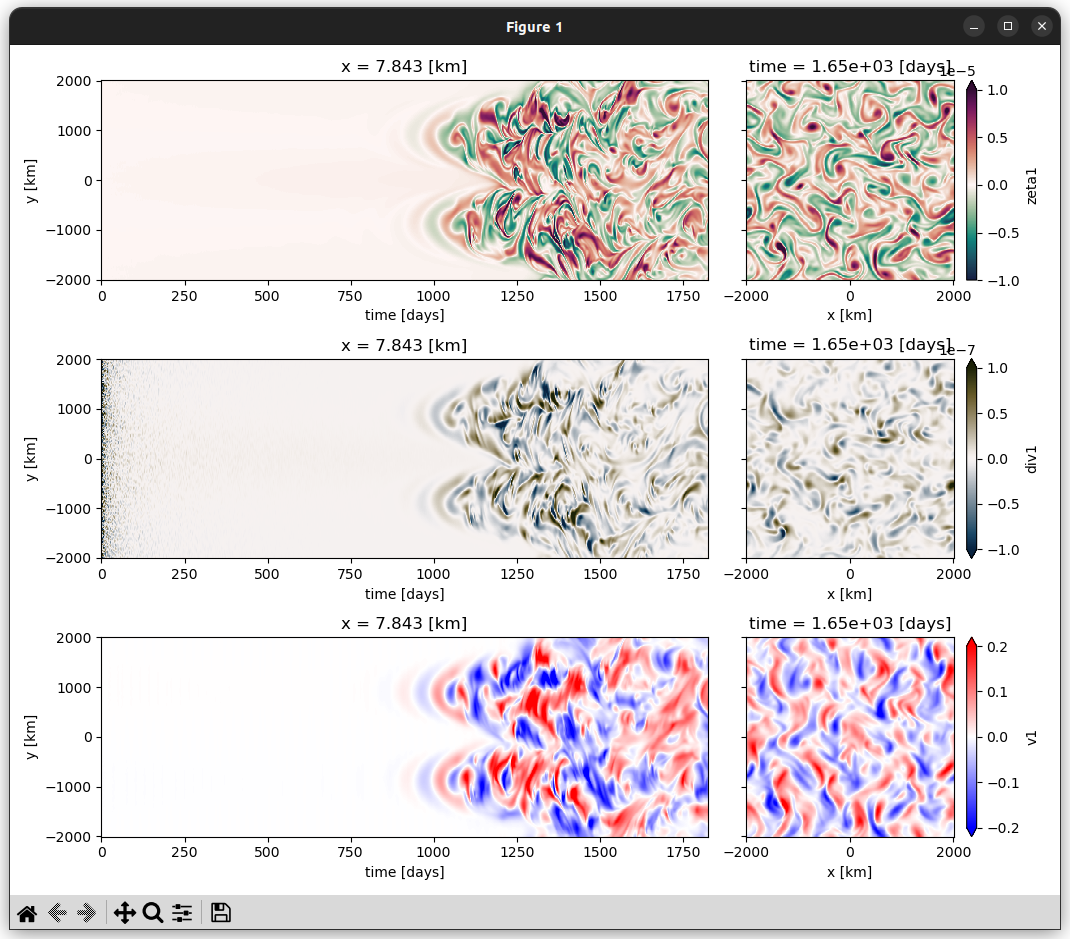
\includegraphics[width=.9\linewidth]{figures/tests/test_SW_2023-03-18.png}
\caption{\label{fig:org769c48b}Résultat du test de qualité du modèle. En ordre, diagramme de Hovmoller de la divergence, du rotationnel et du courant dans la première couche.}
\end{figure}
\end{document}
